\documentclass[12pt,a4paper]{article}

% Options possibles : 10pt, 11pt, 12pt (taille de la fonte)
%                     oneside, twoside (recto simple, recto-verso)
%                     draft, final (stade de développement)

\usepackage[utf8]{inputenc}   % LaTeX, comprends les accents !
\usepackage[T1]{fontenc}      % Police contenant les caractères français
\usepackage[french,english]{babel}  % Placez ici une liste de langues, la
                              % dernière étant la langue principale
\usepackage{textcomp}		  % pour le caractère ° and ~     
\usepackage[normalem]{ulem}   % pour rayer le texte
\usepackage{textgreek}		  % lettres grecs sans avoir à enter en math mode

%vector font
%\usepackage{cm-super}
 
%nested enumerate
\usepackage{enumitem}

%Abstract > Summary
\addto{\captionsenglish}{\renewcommand{\abstractname}{English and French abstract}}

%Figures                    
\usepackage{graphicx}
\graphicspath{ {Figures/} }
\usepackage{float} %To prevent floating figure
\usepackage[a4paper,left=2.5cm,right=2.5cm,top=3.0cm,bottom=3.0cm]{geometry}% Réduire les marges
\usepackage{titlesec} % Modifier le style des sections et chapitres

%Caption
\newcommand{\jcaption}[2]{\itshape \caption[#1]{\itshape #1#2}}

%Tableau
\usepackage{array,multirow,tabularx} % For table
\usepackage{slashbox} % Pour couper les tableaux avec une ligne diagonale
\usepackage[font=small,labelfont=bf]{caption}
\newcolumntype{L}[1]{>{\raggedright\let\newline\\\arraybackslash\hspace{0pt}}m{#1}}
\newcolumntype{C}[1]{>{\centering\let\newline\\\arraybackslash\hspace{0pt}}m{#1}}
\newcolumntype{R}[1]{>{\raggedleft\let\newline\\\arraybackslash\hspace{0pt}}m{#1}}

%paragraph
\setlength{\parindent}{4em}
\usepackage{indentfirst}
\setlength{\headheight}{15pt}
 
%list
\newenvironment{myitemize}
{ \begin{itemize}
	\setlength{\itemsep}{0pt}
	\setlength{\parskip}{0pt}
	\setlength{\parsep}{0pt} }
{ \end{itemize} }


\newenvironment{myenumerate}
{ \begin{enumerate}
	\setlength{\itemsep}{0pt}
	\setlength{\parskip}{0pt}
	\setlength{\parsep}{0pt} }
{ \end{enumerate} }
 
%Référence
\usepackage{hyperref }
%Référence perso
\newcommand{\refperso}[2]{\hyperref[#2]{#1~\ref*{#2}}}
%tilde
\newcommand{\tildep}[0]{\raise.17ex\hbox{$\scriptstyle\sim$}}

\usepackage{fancyhdr} % for use of \pageref{LastPage}
\pagestyle{fancy}

% Modifie le style par défaut
\fancypagestyle{IHA-fancy-style}{%
  \fancyhf{}% Clear header and footer
%  \fancyhead[L]{\leftmark}
%  \fancyhead[R]{\rightmark}
  \fancyhead[C]{\rightmark}
  \fancyfoot[L]{Jonhathan Pinon}
  \fancyfoot[R]{Page : \thepage}% Custom footer
  \renewcommand{\headrulewidth}{0.4pt}% Line at the header visible
  \renewcommand{\footrulewidth}{0.4pt}% Line at the footer visible
}

%Formules mathématiques centrées avec espace
\newenvironment{sp_equation}
{ \begin{equation}
 }
{ \end{equation} \smallskip }

%Appendix
\usepackage[titletoc,toc,page]{appendix}
%\renewcommand{\setthesubsection}{\Alph{section}}

%Scientific form in text mode
\newcommand{\sfnb}[2]{#1 $ \times$ 10 \textsuperscript{#2}}

%Math
\usepackage{amsmath,amssymb,mathrsfs}

\sloppy                       % Ne pas faire déborder les lignes dans la marge

\begin{document}
%

\begin{titlepage}

\vspace{5 cm}

\begin{center}

\Huge Final report for the peer-graded assignment of capstone project

\vspace{3 cm}

\Huge \textbf{Identifying the best places to open a French restaurant in Nagoya}

\vspace{2 cm}

\Large \textbf{by Jonhathan Pinon} \\

\vspace{2 cm}


\large 15/07/2019


\end{center}

\end{titlepage}

\clearpage
\tableofcontents
\phantomsection

\listoffigures


\pagestyle{IHA-fancy-style}


\section{Introduction}

\subsection{Background}


Nagoya is one of the largest cities in Japan. It has a population of over 2 million and is situated in the middle-eastern part of Japan. In Japan, French cuisine is relatively popular. According to Foursquare data, there are about a hundred of French restaurants in Nagoya. Supposing that a chain of restaurants specialized in French cooking want to open new French restaurants in Nagoya, where would be the best places? 

\subsection{Problem}

The best place is the place that would attract the most customers. In this report, we define popularity as the number of customers. Ideally, we would need to identify, and ideally quantify, which factors are beneficial for attracting customers, and which are not. For example, we can expect the proximity of subway station to substantially increase the popularity. On the other hand, we can expect that similar restaurants would decrease the popularity. However, the lack of data make quantifying the factors impossible. We will still attempt to estimate the best places using other means.

\subsection{Interest}

Such a map would obviously be very interesting for any group who wishes to open a restaurant. A restaurant popularity depends on its quality, but the location is still a major factor. To maximize potential income, choosing the place that would potentially attract the most customers is very important.

\section{Data description}

\subsection{Data sources}

Foursquare location data is the only data source. Foursquare provides the position of most restaurants, train stations, subway stations, and other venues in Nagoya. The location of all venues in Nagoya listed by Foursquare, along with their category, will be our main data during this study. We could further increase the amount of data using other API such as Google Maps's API, but we judged it would create more inconsistently than benefits due to the different nature of the data (for example, the categories are not the same). Henceforth, we limited our source to Foursquare.

\medskip

In addition, Foursquare provides stats about each venue such as the number of visitors currently at the specified venue. By collecting the number of users at a specific venue over the course of several weeks, we could get an estimate of its popularity. Unfortunately, in the scope of this course, we did not have enough time to collect enough data.  Foursquare allowed developers to get the total number of visits of any venue by getting the details of that venue, thanks to the response field \textit{checkinsCount}, but since April 2018, this no longer possible (reference 1).

\subsection{Dataframes}

Almost all data are stocked in dataframes, objects of the library pandas. Some data were stocked temporary in lists and Series for the sake of coding.
All relevant data from Foursquare were stocked into just two dataframes. A dataframe containing all French restaurants in Nagoya (Figure \ref{french_df}), and a dataframe containing all venues in Nagoya (Figure \ref{nagoya_df}).

\begin{figure}[ht]
	\begin{center}
			  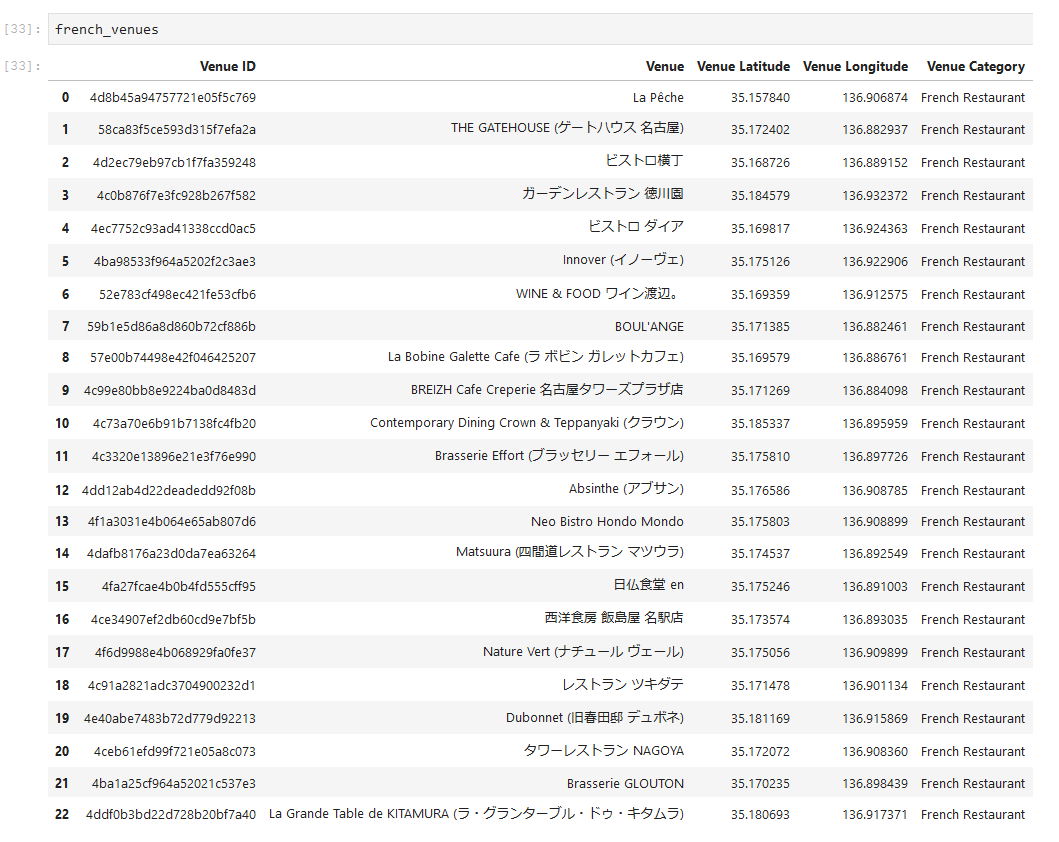
\includegraphics[width=15cm]{french_venues_df.png}
	\end{center}
	\caption [\itshape First part of the dataframe listing all French restaurants in Nagoya]{\itshape First part of the dataframe listing all French restaurants in Nagoya}	
	\label{french_df}
\end{figure}

\begin{figure}[ht]
	\begin{center}
			  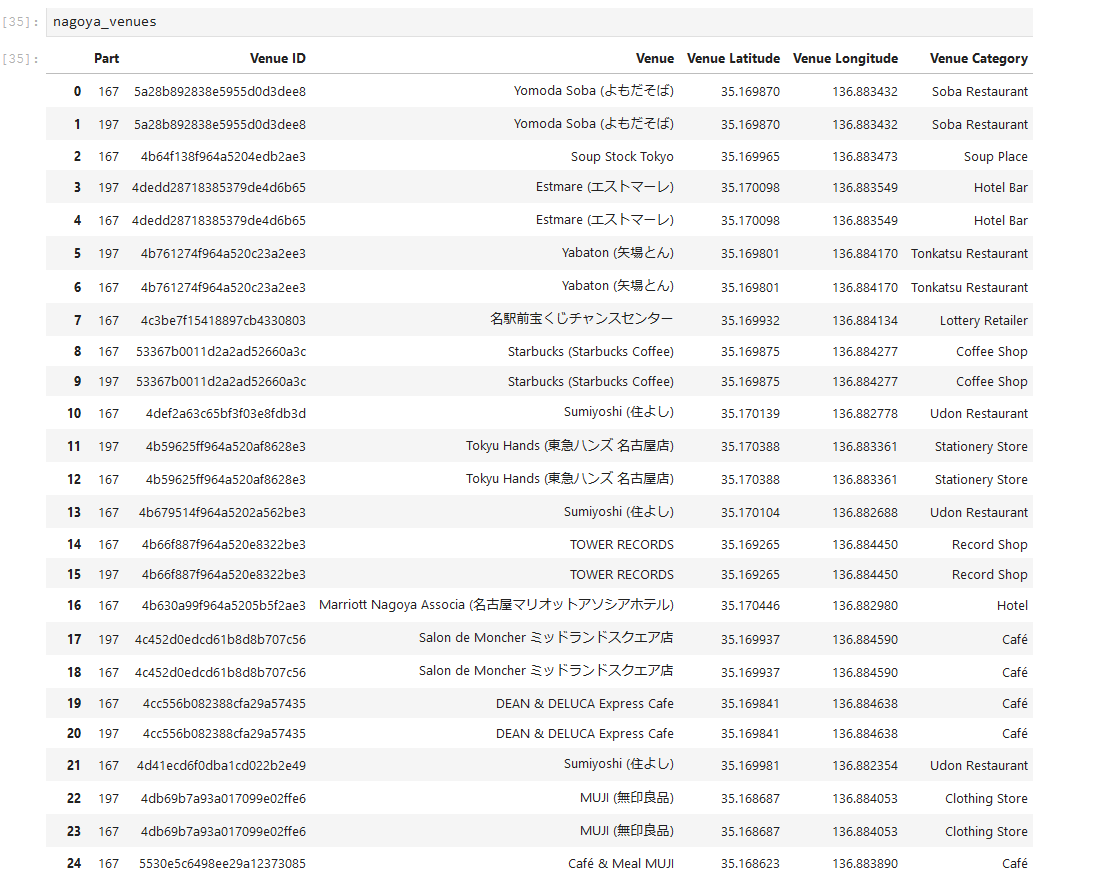
\includegraphics[width=15cm]{nagoya_venues_df.png}
	\end{center}
	\caption [\itshape First part of the dataframe listing all venues in Nagoya]{\itshape First part of the dataframe listing all venues around French restaurants in Nagoya}	
	\label{nagoya_df}
\end{figure}


\subsection{Data cleaning}

In the case of the dataframe containing the French restaurants, \textit{french\_venues}, directly after the construction of the dataframe from Foursquare data, some venues are not classified as French restaurants. This is because in Foursquare, venues can have several categories. When searching for all venues belonging to a certain category, Foursquare will pick all venues that contains that specific category among all their categories. Then, in our script, for each venue, we select its first category as its category which will be later stocked in the dataframe. As that first category may not necessarily be 'French restaurant', we manually reassign the category 'French restaurant' to all venues in \textit{french\_venues}.

\medskip

In the case of the dataframe containing all venues around French restaurants in Nagoya, due to how we collected the data, there are thousands of duplicates. We remove them by dropping the duplicate rows from the dataframe. The construction of that dataframe, \textit{nagoya\_venues}, is explained in details in the following section.

\section{Methodology}

\subsection*{Principe}

Our final goal is to get a list of the best places to open a French restaurant in Nagoya. As mentioned above, we cannot measure the popularity of a restaurant using Foursquare data. Consequently, it is nearly impossible to find out and measure what factors, related to its geographical position, make a restaurant popular. 

\medskip

Let us think from another perspective. Let us assume the owners of the already existing French restaurants thought thoroughly where they should open a French restaurant. Let us assume that the previous French restaurants were opened at \textit{a good place}. Then by analyzing the geographical details of each French restaurant, we can estimate in what kind of places French restaurants tend to be opened. In other words, which are the best places to open a French restaurant. By \textit{geographical details}, we mean the venues surrounding the French restaurants. For example, if we discover that French restaurants tend to be close to subway stations and far away from other restaurants, then we find the best places in Nagoya by looking at which points the distances from subway stations are minimized while the distances from other restaurants are maximized. 

\medskip

This is the general idea of our methodology. Due to the limiting computing power, we cannot look at each possible point (i.e: set of longitude and latitude) in Nagoya. We decided to limit our study to a grid of 30*30 points in an area which contains all French restaurants in Nagoya. There are thus 900 points in the grid. One part of the grid is shown on Figure \ref{nagoya_grid}. The red circle is the area studied, which was defined so as to contain all French restaurants in Nagoya and their surrounding venues. The meaning of the blue circles is explained in the next subsection. 

\begin{figure}[ht]
	\begin{center}
			  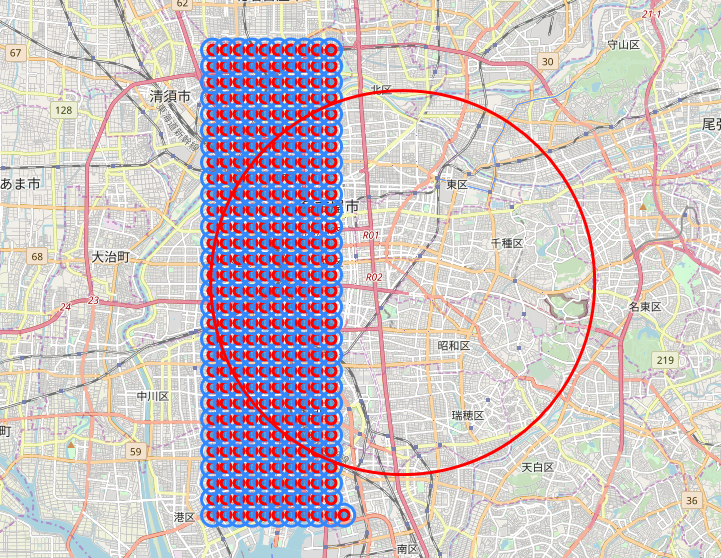
\includegraphics[width=15cm]{nagoya_grid.png}
	\end{center}
	\caption [\itshape Division of Nagoya into a 30*30 grid]{\itshape Division of Nagoya into a 30*30 grid}	
	\label{nagoya_grid}
\end{figure}

\medskip

For each point in the grid, we will calculate a \textit{recommendation index}. The higher it is, the more recommended it is to open a restaurant at that place. This \textit{recommendation index} is the weighted sum of a \textit{similarity index} and a \textit{penalty index}. For each point, the \textit{similarity index} represents how the venues around that point are similar to the venues that tend to be found around French restaurants. The \textit{penalty index} represents the proximity of French restaurants. We assume that it is better to open a French restaurant away from other French restaurants due to competition.

\begin{equation}
	\textbf{recommandation}_{i} = (1 - c) * \textbf{similarity}_{i} - c * \textbf{penalty}_{i}
\end{equation}

$c$ is a coefficient used to weight the importance of the similarity versus the penalty. It is calculated later.

\subsection{Preparation of the data}

The collection of all French restaurants in Nagoya is straightforward. We run a single request to Foursquare API to get the list of all venues that are classified as \textit{French restaurant}. The latitude and the longitude of the center of the circle where the venues are explored are obtained through the python libray \textit{geopy}.

\medskip

The collection of all venues, which are NOT French restaurants, is more complex. One of the limits of Foursquare API is that a single request, to explore the venues around a place, only gives back at most 100 venues. However, there are certainly more than 100 venues in Nagoya. To get as many venues as possible, we split Nagoya, or more precisely the area around the French restaurants, into 900 parts, in a 30*30 grid. The grid is the same grid referenced in Figure \ref{nagoya_grid}. Then for each area, we make a call and get the list of all venues in that area. The blue circles in the Figure represent the size of each area. Let us notice that all area inside the red circle, which contains all French restaurants in Nagoya, is covered by the blue circles. Thanks to this division of Nagoya, we can get most of the venues around French restaurants by making 900 calls to Foursquare API.

\medskip

Of course, collecting the venues this way will generate a lot of duplicates. Indeed, each point inside the red circle is covered by several blue circles. To clean our data, we drop the duplicates in \textit{nagoya\_venues}.

\medskip

The calculation of the \textit{similarity index} will involve millions of mathematical operations. The distance between each French restaurant and each venue in Nagoya will be calculated. We can calculate the distance between two points on Earth using the Haversine formula, but this formula involves trigonometric functions which would make the computational time far too long (more than one day). To accelerate as much as possible the calculation of the \textit{similarity index}, we will first calculate the position of all venues (including French restaurants) in a local Cartesian system. The center of this coordinate system will the center of the red circle, shown on Figure \ref{nagoya_grid}. To transform the latitude and longitude into Cartesian coordinates, we use the formula described in reference 2. This formula is derived from the Equirectangular approximation. The formula is as follow:

\begin{equation}
	x = R * (lgt - lgt_0) * cos (lat_0)	
\end{equation}

\begin{equation}
	y = R * (lat - lat_0)
\end{equation}

where:

\begin{itemize}
  \item $R$ is the radius of Earth (~6373 km)
  \item $lgt$ is the longitude in radians of the given point
  \item $lat$ is the latitude in radians of the given point
  \item $lgt_0$ is the longitude in radians of the origin
  \item $lat_0$ is the latitude in radians of the origin
\end{itemize}
 
The Equirectangular approximation is a good enough approximation considering the distances involved. We verified this hypothesis by comparing the distances calculated using this approximation to the distances calculated using the Haversine formula.

\medskip

All venues in \textit{french\_venues} and \textit{nagoya\_venues} have now their coordinates in the local Cartesian system.
 
\subsection{Calculation of the recommendation index}

\medskip

The \textit{recommendation index} is the weighted sum of the \textit{similarity index} and the  \textit{penalty index}. 
The \textit{similarity index} is calculated as follows: 

\paragraph{Step 1 : 100 closest venues for each French restaurant}
For each French restaurant in \textit{french\_venues}, get the 100 closest venues (which are not French restaurants). The venues are obtained from \textit{nagoya\_venues}.The distances are calculated using the Cartesian coordinates. The 100 closest venues along with the distances to the French restaurant are saved into a dataframe. The list of dataframes is called \textit{french\_100venues\_list}. We now have a list of dataframes which show what venues are found near French restaurants. More importantly, we have the distance of each French restaurant to their closest venues.

\paragraph{Step 2 : construction of the super french restaurant model}
Concatenation of all dataframes in \textit{french\_100venues\_list} into a super dataframe, called \textit{model\_fr}. What matter are the distance and the venue category of each row. All venues inside that dataframe will be compared to the 100 closest venues of each point in the grid. In a way, the super dataframe is like the average venues found near a French restaurant.

\paragraph{Step 3 : 100 closest venues for each point in the grid}
Like it was done with the French restaurants, we create a list of dataframe, called \textit{nagoya\_100venues\_grid}. Each dataframe in the list contains the 100 closest venues to a specific point of the grid. After the dataframes are created, we calculate the minimum distance of the maximum distance found in each dataframe. In other words, we get the minimum distance among the distance between the 100 farthest venue and the respective point. This value, called \textit{max\_distance\_normalization} is an important part of the model. The meaning of this value will be explained shortly.

\paragraph{Step 4 : extrapolate each dataframe of the grid to compare it to \textit{model\_fr}}
Each point of the grid is associated with 100 venues, yet \textit{model\_fr} have $100 * number \ of \ French \ restaurants$ venues. To compare the two dataframes, we extrapolate the dataframe in \textit{nagoya\_100venues\_grid}. For each dataframe, we duplicate X times each venue inside that dataframe. X is the number of restaurants.

\paragraph{Step 5 : calculation of \textit{similarity index}}
We compare each extrapolated dataframe, \textit{nagoya\_ex\_100venues}, to \textit{model\_fr}. We define the similarity between a venue of \textit{nagoya\_ex\_100venues} and a venue of \textit{model\_fr as follow:

\begin{equation}
	similarity = - abs(distance_{ng} - distance_{fr})
\end{equation}

where:
\begin{itemize}
  \item $distance_{ng}$ is the distance of between the venue in \textit{nagoya\_ex\_100venues} and the point of the grid.
  \item $distance_{fr}$ is the distance of between the venue in \textit{model\_fr} and the respective French restaurant
\end{itemize}

If $distance_{ng}$ = $distance_{fr}$ then the similarity is maximum. It means that the venue in \textit{nagoya\_ex\_100venues}, relative to the point of the grid, is placed just like the venue in \textit{model\_fr}.

The formula above is in fact applied only if:

\begin{itemize}
  \item The two venues compared belong to the same category
  \item The absolute difference of the two distances is lower than \textit{max\_distance\_normalization}. 
\end{itemize}

In the cases, we define $similarity$ as equal to \textit{max\_distance\_normalization}. Let's explain the meaning of this value. When we constructed  \textit{nagoya\_100venues\_grid}, we took the 100 closest venues. It means that we may have missed venues commonly found near French restaurants, that could be just a little farther away from the 100th closest venue. If we take into account the fact that the density of venues differ, then we realize we must add \textit{max\_distance\_normalization} into the model. Let's why by using a more concrete example:

\medskip

There are two points. For both points, we get the 100 closest venues. In the first case, as the point is situated in a low-density area, the 100th closest venue is 2000 meters away from the point. In the second case, as the point is situated in high-density area, the 100th closest venue is 200 meters away from the respective point. Now, let's imagine there is a venue, commonly found near French restaurants, just beside the 100 closest venue in the second case, so let's say 201 meters away. Then if we don't 

\section{Results}

\section{Discussion}

\section{Conclusion}

\section*{References}

\begin{enumerate}
  \item https://developer.foursquare.com/docs/announcements\#start-up-tier-launch
  \item http://www.movable-type.co.uk/scripts/latlong.html
\end{enumerate}


\end{document}


